6. По теореме Виета $x_1+x_2=-9,\ x_1x_2=q.$ Тогда $\cfrac{1}{x_1}+\cfrac{1}{x_2}=\cfrac{x_1+x_2}{x_1x_2}=\cfrac{-9}{q}=-\cfrac{1}{2}\Rightarrow q=18.$ Построим параболу $x^2+9x+18$ по трём точкам $(-3;0),\ (-6;0),\ \left(-\cfrac{9}{2}, -\cfrac{9}{4}
ight).$
$$\begin{tikzpicture}[scale=0.5]
\begin{axis}[
    axis lines = middle,
    grid=major,
    legend pos={south west},
    xlabel = {$x$},
    ylabel = {$y$},
    %ymin=-80,
    %ymax=250,
    xtick={-10, -7, -6, -4.5, -3, 1},
    xticklabels={-10,-7, -6, $-\cfrac{9}{2}$, -3, 1},
    ytick={28,4,-2.25},
    yticklabels={28,4,$-\cfrac{9}{4}$}             ]
	\addplot[domain=-10:1, samples=100, color=black] {x*x+9*x+18};
%\addplot[domain=-3.1:2.5, samples=100, color=red] {70*abs(1-2*abs(abs(x)-2))-10*x^2+10*x-70};
	%\addlegendentry{$\text{Рис. 1}$};
\end{axis}
\end{tikzpicture}$$
